\chapter{Machine learning approach}
\label{ch:MachineLearning}
\graphicspath{{Chapter4/Chapter4Figures/}}

The previous chapter briefly described the basic workings of the optical mark recognition system inside the automatic test grader. There is still one critical piece of evidence that has not yet been observed in this basic system. This information is the characters that the student writes in the designated boxes.

\nomenclature[A]{$DCNN$}{Deep convolutional neural network}
This next chapter will provide two machine learning approaches to significantly improve the accuracy in identifying digits over the previous standalone basic system, discussed in Chapter \ref{ch:ImageProcessing}. An approach to locate and classify handwritten characters, provided by the students, using a deep convolutional neural network (DCNN), is described. Next, a more accurate method in estimating the  student answers and student number, using probabilistic  graphical models (PGM), is also discussed. 

\section{Character recognition using a neural network}

This section focusses on processing the characters that the students write down in the designated boxes, as shown in Figure \ref{fig:sa}. A machine learning approach, called a neural network, is implemented to process these digits. This neural network can take an input of a 28 by 28 dimensional array of floating point numbers. These numbers represent a 28 by 28 greyscaled image that includes the digit being classified. The neural network is then tasked with calculating the probability of each digit being present in the particular image. Before each digit can be classified using a neural network, the individual 28 by 28 greyscaled image must first be found for each digit inside the test sheet. Image processing is required to achieve this, as described in the next section.
\begin{figure}
  \centering
  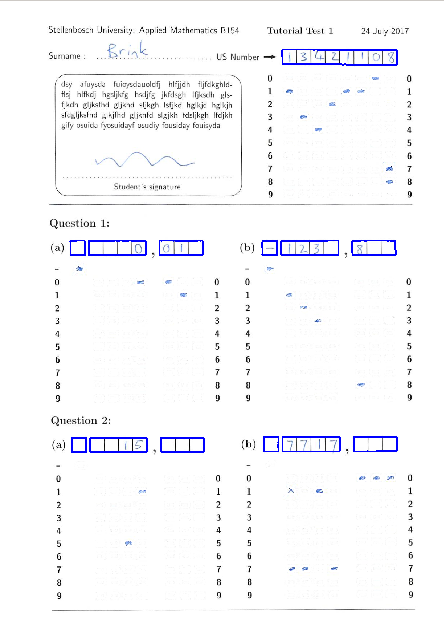
\includegraphics[width=6cm]{DigitScan}\\
  \caption{Image showing found contours for boxes used for character recognition.}
  \label{fig:sa}
\end{figure}

\subsection{Preprocessing and creating digit images}
\label{sec:preprocess}

In order to generate a 28 by 28 pixel image for each digit, the system must first find the location of each digit. Once this is done, the digits is processed and a corresponding 28 by 28 image, best representing that digit, can be created. This is done in the following 6 steps as seen below:

\begin{enumerate}
\item Find the contour closest to the expected location of the block, calculated in Section \ref{sec:findTemplate}. This is illustrated in Figure \ref{fig:sa}. It can be seen that the bubbles are already processed.

\item Transform the image to become fully rectangular using OpenCV's $four\_point\_transform$ method. This method applies a four point perspective transform on the image to reshape it into a rectangular form. An example of the final product can be seen in Figure \ref{fig:bp}.

\begin{figure}
  \centering
  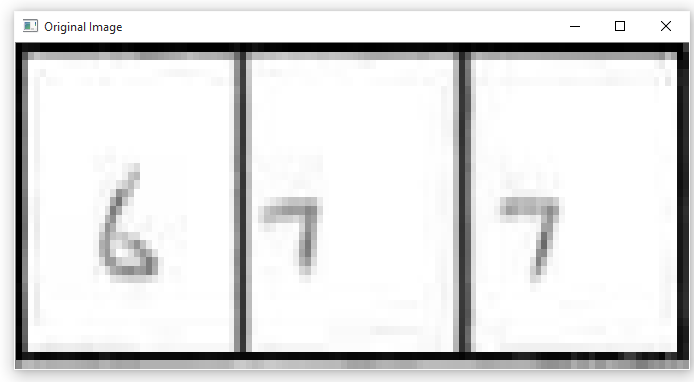
\includegraphics[width=7cm]{BeforeProcessing}\\
  \caption{The box contour found is normalized to form a rectangular shape.}
  \label{fig:bp}
\end{figure}

\item Perform a Radon transform on the image, at an angle of 0$^{\circ}$ and 90$^{\circ}$ to find the dark lines in the blocks. These lines are then removed from the image, as shown in Figure \ref{fig:ar}. 

\begin{figure}
  \centering
  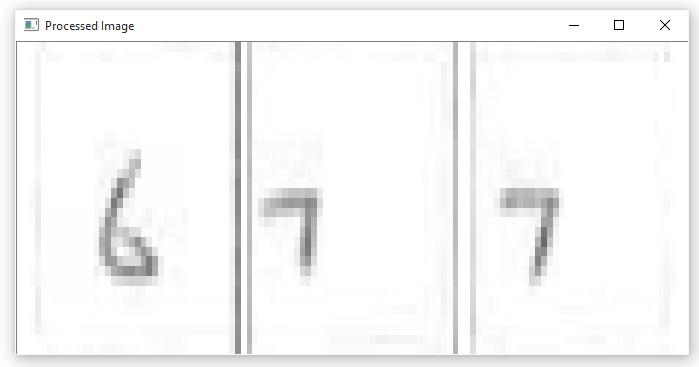
\includegraphics[width=7cm]{AfterRadon}\\
  \caption{Box after black lines gets filtered out, found using a Radon transform.}
  \label{fig:ar}
\end{figure}

\item Use the indexes received from the Radon transform, of the positions of original black lines, to segment the image into the different boxes.
\item A custom segmentation algorithm is used to find the pixels most likely to belong to the digit. This algorithm is developed and implemented using a breadth first search technique to cluster the image into different segments. The algorithm works by first searching the image for pixels higher than a specific threshold value. This value specifies if an pixel is background or belongs to an object. Then all the pixels higher than the threshold value gets assigned to a segment. A segment is thus classified as a local region that does not connect to any other segment through pixels higher that a threshold. The segment that most likely represents the digit is then extracted, as shown in Figure \ref{fig:c}.
\begin{figure}
  \centering
  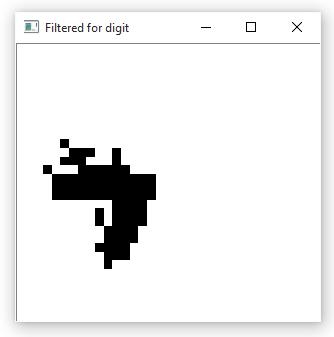
\includegraphics[width=5cm]{Cluster}\\
  \caption{Custom segmentation algorithm used to find the main cluster in the remaining image.}
  \label{fig:c}
\end{figure}

\item The area that the segment occupies is then calculated, as shown in Figure \ref{fig:areaLoc}.

\begin{figure}
  \centering
  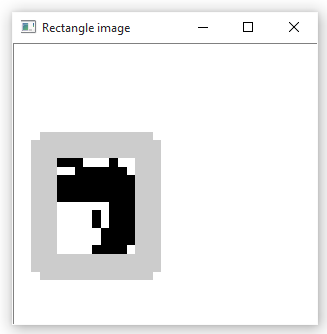
\includegraphics[width=5cm]{DetectArea}\\
  \caption{Area block drawn around the segment most probable to belong to the digit.}
  \label{fig:areaLoc}
\end{figure}

\item Next the image is centred and normalized using the image area as reference.  This is shown in Figure \ref{fig:final}.

\begin{figure}
  \centering
  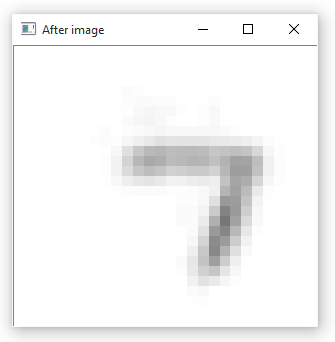
\includegraphics[width=5cm]{TranslateAndScale}\\
  \caption{Image after final translation and normalization is applied.}
  \label{fig:final}
\end{figure}

\item The image is then reshaped into a 28 by 28 greyscaled image to be processed by the neural network.
\end{enumerate}
As mentioned, a 28 by 28 greyscaled image is used as input. Thus if each pixel represents one value, ranging from 0.0 to 1.0, there is total of 748 input values. Each digit image is thus represented by  one of these 28 by 28 greyscaled images. These 784 numbers is now used as input to a neural network to predict the digit. An overview of this neural network will be given next.

\subsection{Classification of digits}

A neural network is a powerful machine learning tool for approximating complex functions. The basic architecture of a neural network is illustrated in Figure \ref{fig:nn}. These networks are simplified approximations of how neurons in the brain works. Each neuron in the network acts as a small processing unit that can take a input and produces an output. The power of a neural network lies in that fact that these neurons have internal values that can be tweaked depending on the characteristics the user wants the network to approximate. This therefore allows complex functions to be trained onto such networks.

For this project, a neural network is trained to estimate the probability of which of the 10 digits, from 0 to 9, are most likely present in the input image. The neural network will take a two dimensional array, representing a greyscaled image, as input to the network. Figure \ref{fig:mnist} illustrates an example input of a neural network using a 14 by 14 example image. For this project a 28 by 28 image is used. In the next section the basics of these neural networks are discussed.

\begin{figure}
  \centering
  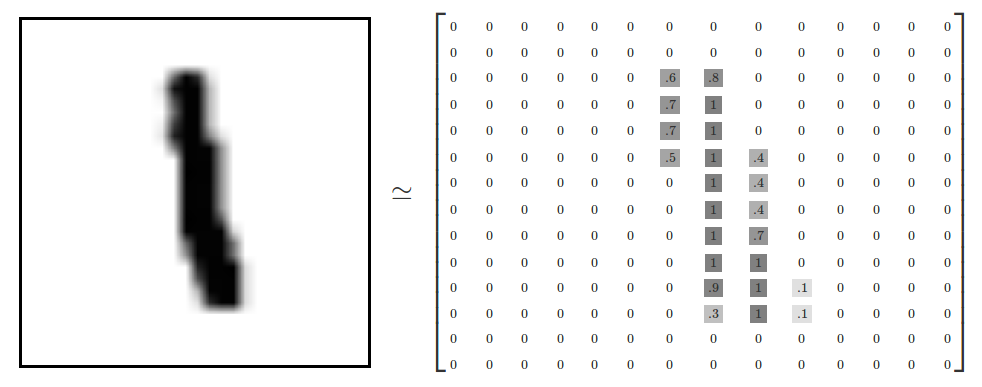
\includegraphics[width=10cm]{MNIST}\\
  \caption{Example image used as input to the neural network, from \citet{tensor2017}}
  \label{fig:mnist}
\end{figure}

\begin{figure}
  \centering
  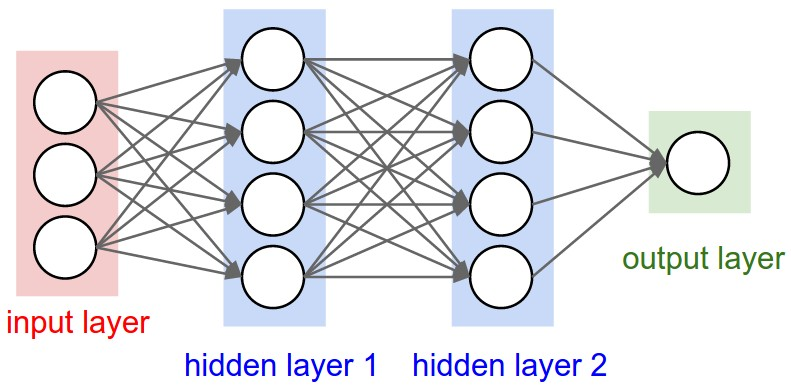
\includegraphics[width=10cm]{NN}\\
  \caption{Basic structure of a neural network, from \citet{karpathy2017}}%, 
  \label{fig:nn}
\end{figure}

\subsubsection{The Neural Network basics}

The neuron unit is a small processing unit and by including many of these neurons a neural network can be built. Neural networks consist of input, hidden and output layers (\citet{MichealN2015}). This network works by first assigning values to the input layer of the network. For this project those values are the 784 values received from the digit image. The network then sends signals through the network and generates an output. A breakdown of a neural network will be given next.

\subsubsection{The Artificial Neuron}
Each neuron in the network takes in a list of input values. These input values are given by the output values of the neurons in the previous layer, illustrated in Figure \ref{fig:nn}. These values are then multiplied by internal weights of the neuron and a final weight, named the bias, is then added. These internal weights are therefore fixed to a specific value, depending on what function that neuron tries to approximate. A bias variable is also added to expand the range of functions a neuron can approximate. The weighted sum of these inputs are then added with the bias variable to give,
\nomenclature[S]{$x_{i}$}{Input value at index $i$}
\nomenclature[S]{$w_{i}$}{Weight value at index $i$}
\nomenclature[S]{$b$}{Bias variable added to allow a neuron to have an offset in its output}
\nomenclature[S]{$z$}{Weighted sum of a neuron's inputs and internal variables}
\nomenclature[S]{$z_k$}{Weighted sum of a neuron's inputs and internal variables at index $k$ in the specific layer}
\nomenclature[S]{$k$}{Index value for a specific input neuron}
\nomenclature[S]{$c$}{Number of inputs to a neuron}
\begin{align}
  z =  &\displaystyle{\sum_{i=0}^{c} x_{i}*w_{i} + b}.
\label{eqn:nnOut}
\end{align}
In Equation \ref{eqn:nnOut}, $c$ is the number of inputs and $x_{i}$ and $w_{i}$ are the input and weight values at index $i$. The bias term, $b$, enables an offset in the output, $z$, of the neuron.
The summed value then gets normalize using an sigmoid function,
\nomenclature[S]{$\sigma(z)$}{Normalization function in a neural network}
\begin{align}
  \sigma(z) =  &\displaystyle{\frac{1}{1 + e^{-z}}}.
\label{eqn:sigmoid}
\end{align}
The artificial neuron therefore takes in a weighted input with a bias and produces a normalized output $\sigma(z)$. By adjusting the weights and bias variable, each neuron can learn to exhibit certain characteristics. This process allows different functions to be approximated by adjusting these variables. If a network of these neurons is used together, as illustrated in Figure \ref{fig:nn}, complex functions can be trained onto the network. In this project these weights and biases need to be set to specific values, to allow the network to accurately categorize digits from an image.

\subsubsection{Generating an output from the network}
After the 748 input values have been assigned to the network inputs, each of the network's layers can be calculated consecutively. This is done using Equations \ref{eqn:nnOut} and \ref{eqn:sigmoid} on each layer consecutively, starting at the first hidden layer. Once the first layer's outputs are calculated, the next layer can be calculated. This process is repeated until all the layers are calculated. After this step, the final values can be read from the output neuron that represents the result. In this project ten output neurons are used to represent the likelihood of each of 10 digits, given the input data. The output neurons are then turned into probabilities by normalizing these outputs using

\nomenclature[S]{$p(i)$}{Probability of digit at index $i$}

\begin{align}
  p(i) =  &\displaystyle{\frac{\sigma(z_{i})}{\sum_{k=0}^{10} \sigma(z_{k})}},
\label{eqn:normal}
\end{align}
where $p(i)$ is the probability of a digit and $i$ being an index for each digit. The value $\sigma(z_{i})$ represents the values of the output neuron at index $i$.

\subsubsection{Deep Convolutional Neural Network}

The previous section gave an overview of a basic neural network implementation. In recent years much more powerful neural networks such as Deep Convolutional Neural Network (DCNN) have been introduced. A DCNN uses the basic principles described above, but has extra optimized features that allow a neural network with many layers to be constructed and trained. The exact mathematics behind these Deep Neural Networks are beyond the scope of this project report. This neural network is implemented in TensorFlow (\citet{Tensor}) and allows a neural network to achieve highly accurate results on classifying digits. For this project a neural network optimized for digit classification, as described in \citet{Tensor}. The neural network was only adjusted to increase its accuracy for this specific grading system. These results are described in Chapter \ref{ch:Results}.

\subsubsection{Training of the neural network}
\label{sec:trainNN}
The MNIST dataset is used to train the DCNN neural network (\citet{mnist}). This is a database that has a labelled training set of 60 000 images, and a labelled test set of 10 000 images. For each image in the training set, there is an accompanied label that specifies the digit value. The neural network is then trained to model this training set. This is done by adjusting the network's internal weights so that the network's output better represent the labelled training data, given the input images. The basic idea behind the training method used in a neural network is described in Algorithm \ref{alg:nnTrain}.

\begin{algorithm}[H]
\caption{Overview on training a neural network.}
\label{alg:nnTrain}
\begin{enumerate}
\item Calculate the network's output for each of the training images used in the training round.
\item Obtain the error function of the network, using a formula that compares the true labels of the training image with the estimated labels generated by the network.
\item Calculate the value with which each weight should be changed to reduce the error function. One method of doing this is using gradient decent with back propagation.
\item Repeat steps 1 to 3 until a time or accuracy criterion is met.
\end{enumerate}
\end{algorithm}

Once this process is completed, the network is ready to classify handwritten digits. This produces a probabilistic output of each intended digit in the test sheet. The next step is to incorporate this character evidence with the bubble evidence to produce a accurate estimate of the intended student entries. A method to achieve this is discussed in the next section.

\section{Probabilistic Graphical Models}
\label{sec:PGM}
The final problem the system needs to solve, is to probabilistically determine the most likely student entries given the bubble and character evidence. This is achieved by implementing two probabilistic graphical models (PGM).

\subsection{Overview of the system}
A probabilistic graphical model is a probabilistic graph containing random variables, where the graph expresses the conditional independence structure between these variables. The type of PGM used for this project is a Bayesian network. A Bayesian network models a set of random variables and their conditional dependencies via a directed acyclic graph (DAG).

A graphical model in essence allows a problem to be represented as information (nodes or circles) and relationships (directed arrows). An example of such a graph is shown in Figure \ref{fig:pgmDigit}. The directions of the arrows represent what information causes other information to be created, thus given a parent to offspring interpretation. These graphs allow for intuitive reasoning about how the system should operate. For this project an observation is made in the form of character and bubble evidence. The models are then tasked with inferring the values the student most likely wrote down, given the evidence.

\subsection{Estimating the intended digit}
\label{sec:studentDigit}

\begin{figure}
  \centering
  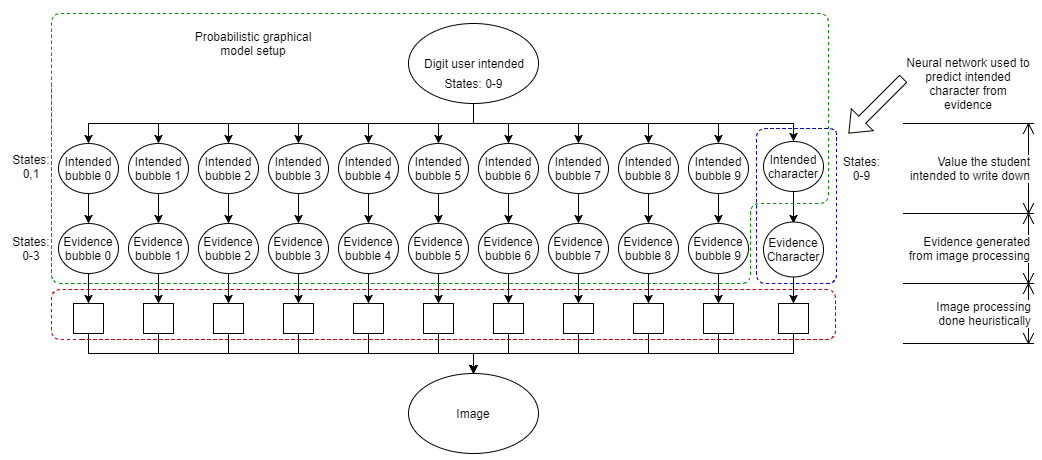
\includegraphics[width=16cm]{pgmDigit}\\
  \caption{Graphical setup for determining the intended digit written by a student.}
  \label{fig:pgmDigit}
\end{figure}

Figure \ref{fig:pgmDigit} should be interpreted in the direction which information flows. Originally a student has a certain digit that he/she wants to portray on the page. This is given by the 'Digit intended' node. There are 10 possible digits to consider and thus the node has 10 possible states. The intended digit then gives rise to character evidence as an image written in a block. Bubble evidence is also produced from the intended digit, but a variable is first introduced in between them. The student might sometimes mistakenly think that the first bubble represents 0 and thus even if the intended digit is 0, the intended bubble might be 1. Thus the intended bubble category also gets introduced, which then produces the bubble evidence, as seen in Figure \ref{fig:pgmDigit}.  

%\begin{figure}
%  \centering
 % 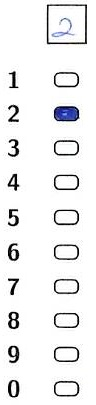
\includegraphics[width=1cm]{column}\\
 % \caption{Column with the evidence that gets considered for the calculation of an intended digit.}
 % \label{fig:column}
%\end{figure}

%When looking at Figure \ref{fig:column}, it is observed that there are 11 evidence areas to consider. 
%They are the the 10 bubbles and the character block. The process of writing down this digit introduces so noise into the system, due to the fact the %student is not always going to write down the digit in exactly the same way. Thus the evidence is also probabilistically linked to the 'intended bubble' %and 'intended character' parent distribution. This evidence then gets written down on the paper and is what ultimately influences how the image looks. %Each of the bubbles can take one of 4 states as evidence. These states are blank, crossed-out, partially coloured in and fully coloured in. The character %block evidence is a 28 by 28 greyscale image. Thus it can have 28*28*256 possible states, where 256 is the possible pixel intensities of each pixel. This %value with true range 0 to 256, gets converted into a normalized value between 0.0 and 1.0 before it gets assigned as inputs to the neural network.

After the model is constructed, the intended digit needs to be estimated, with the image as evidence. This can be done by reasoning from the bottom (image evidence) upwards to the intended digit. The first step is to process the image to produce more tractable evidence. Producing bubble evidence from an image is described in Chapter \ref{ch:ImageProcessing}. In Section \ref{sec:preprocess}, the process to extract the character evidence from the image is also described. Using a neural network the prior probability of each digit can be determined form the character box evidence. The next step is to assign the prior intended digit probability and bubble evidence to a Probabilistic Graphical Model. Using this digit PGM, the intended digit can be inferred.

\subsection{Estimating the student answer}
\label{sec:studentAnswer}

An answers is represented by 8 columns, shown in Figure \ref{fig:stdAns}. The first column represents the sign of an answer. Thus two signs are possible. For each of the remaining 7 columns a number from 0 to 9 can be represented. Thus there are 10 possible values for each of these 7 columns. This gives a possible number of values that an answer can take to be $2*10^7$ equalling 20 000 000. Calculating each of these states are computationally intractable. Thus a assumption is needed to reduce the number of possible states. A fair assumption to make, is that all 20 000 000 possible values are equally likely to be written down. Thus each column digit becomes independent of the other columns' values. This means that if a value in one column is known, it does not influence the probabilities of the other columns having a certain value. Thus the number of states to calculate now becomes $2+10*7$ equalling $72$, because each column's states can now be calculated independently. Knowing this independent property, the student's answer can be calculated by using 7 digit models and a heuristic calculation of the intended sign.

\begin{figure}
  \centering
  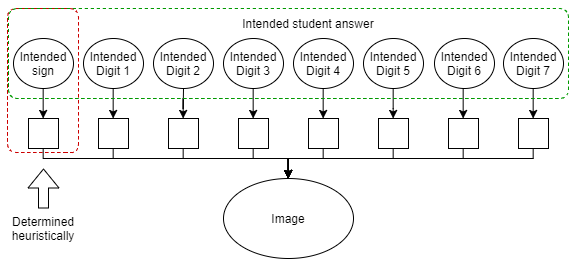
\includegraphics[width=10cm]{ans}\\
  \caption{Graphical setup of student answer.}
  \label{fig:stdAns}
\end{figure}


%In the previous section it was found that determining the intended sign and digit for each column the intended answer can be found. Thus the intended digit for each column is calculated separately using the digit model, as described in Section \ref{sec:intendedDigit}. The intended sign is determined heuristically by using the image processing methods described in Chapter \ref{ch:ImageProcessing} to find if the bubble underneath the sign is coloured in. Once this is done the intended answer is determined by combining the estimated sign and digits in the order seen in Figure \ref{fig:stdAns}.

\subsection{Estimating the student number}
\label{sec:studentNumber}

For the student numbers, knowing one digit value of a column influences the probabilities of the other columns having a certain number. The reason for this is, there are only a limited number of student numbers to consider. Thus if the first digit is a 2, only student numbers starting with 2 still have to be considered. To account for this, an additional node is added above the individual digit probabilities, as seen in Figure \ref{fig:stdNum}. This node represents the probability of each student number being present in the image. The number of states of this node is in the order of $ 900$, depending on the number of student numbers.

Once the graph has been set up, the model can be used to infer the most probable student number. By setting all the bubble evidence and character priors, the student number probabilities can be inferred. This model allows for an accurate result, because student numbers normally differ in more that one digit. The system can thus strongly differentiate between which student number is most likely. It is found that if the student provides only character information with no bubbles coloured in, a highly probable estimate can still be made.

\subsection{Training of a Probabilistic Graphical Model}
In a PGM the conditional probabilities distributions between each random variable that has a relationship (arrow) is needed. In order to calculate these conditional probability distributions training data must be gathered. The previous basic model with the character recognition software is used to estimate the answers for 100 test sheets. Once these sheets where graded the results were manually check. Thus each training label now contained bubble evidence and character proirs from the neural network. With this information, each training set is used to infer the conditional probability needed to train both the digit and student number models. For a mathematically approach to these two PGM models, refer to Appendix \ref{ap:systemOverview}.

\section{Conclusion}
This chapter discusses two machine learning techniques to improve the accuracy with which the system infers the answers written on each scanned test sheet. A method is shown, using a neural network, to estimate the probability of each digit given only the character box as input. Additionally, an approach is discussed, using a PGM, to allow the system to make a final prediction of what the student intended to write down given the image evidence. This PGM method is found to be accurate enough to determine the student number by only using the character recognition information provided.

The following chapter will cover the validation and results of the system from weekly grading done for the Applied Mathematics department.